\documentclass{standalone}
 
\usepackage{tikz}
\usetikzlibrary{graphs}
 
 
\begin{document}
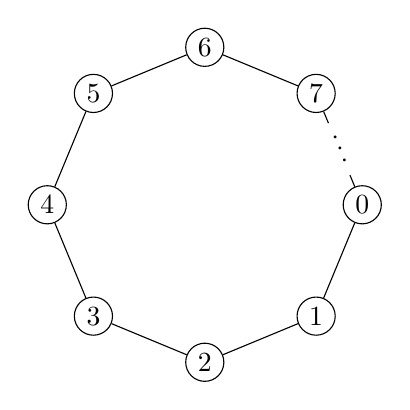
\begin{tikzpicture}
 
    % Create nodes positioned on a circle (nodes are empty)
    \foreach \i [evaluate=\i as \angle using {360/8 * -\i}] in {0,...,7} {
        \node [draw, circle, inner sep = 2pt] (n\i) at (\angle:2cm) {\i};
    }
 
    % Draw edges connecting the nodes in a cycle
    \foreach \i in {0,...,6} {
        \pgfmathtruncatemacro{\next}{\i+1}
        \draw (n\i) -- (n\next);
    }
 
    \draw  (n7) -- node [midway, sloped, fill = white, inner sep = 1.5mm] {$\cdots$} (n0);
\end{tikzpicture}
\end{document}